\documentclass[11pt]{article}
\usepackage[margin=0.9in]{geometry}
\usepackage{amsmath,amssymb,amsthm,mathtools}
\usepackage{graphicx}
\usepackage[colorlinks=true,linkcolor=blue,citecolor=blue,urlcolor=blue]{hyperref}
\usepackage{microtype}

\newtheorem{theorem}{Theorem}
\newtheorem{proposition}{Proposition}
\newtheorem{corollary}{Corollary}
\newcommand{\supp}{\operatorname{supp}}
\newcommand{\E}{\mathbb E}
\newcommand{\K}{\mathcal K}

\title{Two counterexamples in orthogonality\\
of measures and states}
\author{Candidate full-counterexample packet}
\date{11 August 2026}

\begin{document}
\maketitle

\noindent\textbf{Status.}
Candidate full counterexamples; likely valid; human review recommended.

\section{Source questions}

Mejak asks whether, for a separable unital $C^*$-algebra $A$, the common
strong-orthogonal complement of every analytic strongly orthogonal family of
states is comeagre~\cite{Mejak}.  The exact question (PDF page~18) is below.

\begin{center}
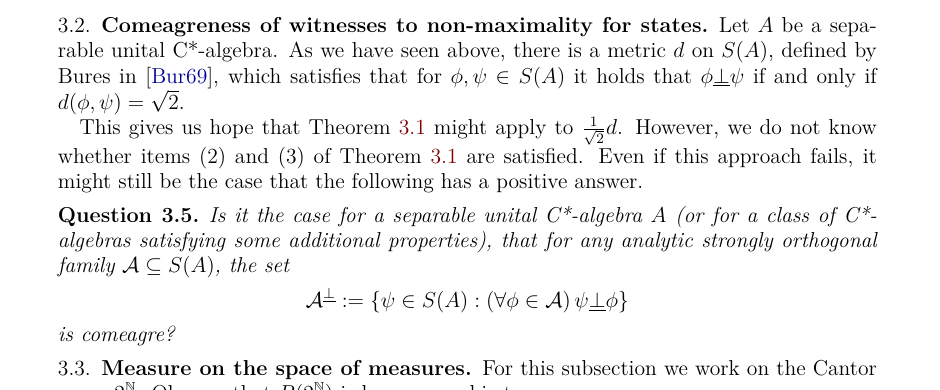
\includegraphics[width=0.94\textwidth]{figures/state_question_crop.png}
\end{center}

The universal statement has a negative answer, already for $M_2(\mathbb C)$
and also for an infinite-dimensional separable unital algebra.

The source next defines a probability measure $\Lambda$ on
$P(2^{\mathbb N})$ by putting independent uniform splitting parameters at
the vertices of the binary tree.  Question~3.6 asks whether
$\Lambda(\mathcal A^\perp)>0$ for every analytic orthogonal family.  Claim~3.7
then asserts $\Lambda(\mu^\perp)<1$ for every fixed $\mu$.  The source passage
(PDF page~19) is reproduced below.

\begin{center}
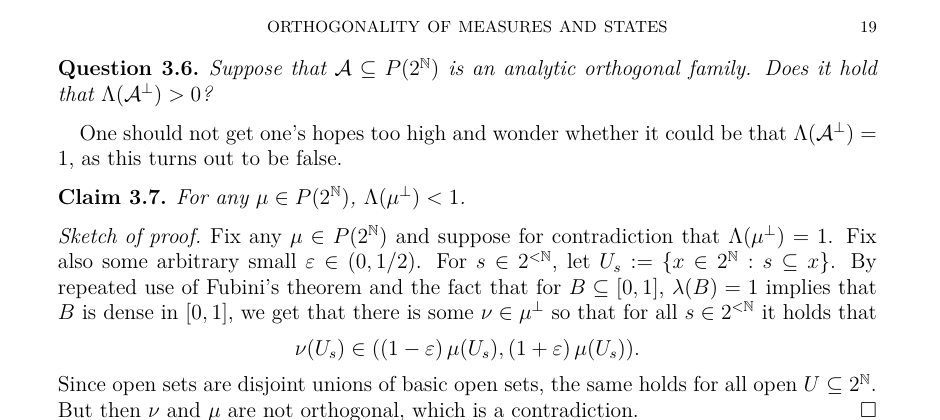
\includegraphics[width=0.94\textwidth]{figures/lambda_question_claim_crop.png}
\end{center}

Claim~3.7 is false: the value is always exactly one.  This also gives a full
and stronger answer to Question~3.6 for every countable family.

\section{Failure of state-space comeagreness}

For a state $\phi$ on $A$, its support is the support projection of its normal
extension to $A^{**}$.  The source defines strong orthogonality by
$\phi\mathbin{\underline\perp}\psi$ if and only if
$(\supp\phi)(\supp\psi)=0$.

\begin{proposition}[full-support obstruction]\label{prop:support}
Let $A$ be a nonzero separable unital $C^*$-algebra.  If $A$ has a state
$\phi$ with $\supp\phi=1$ in $A^{**}$, then the universal assertion in
Question~3.5 is false.  In fact, the closed analytic strongly orthogonal
family $\mathcal A=\{\phi\}$ satisfies
\[
                         \mathcal A^{\underline\perp}=\varnothing.
\]
\end{proposition}

\begin{proof}
A singleton is strongly orthogonal vacuously and is closed in the compact
metrizable state space.  Every state $\psi$ has nonzero support, since
$\psi(1)=1$.  Hence
\[
             (\supp\phi)(\supp\psi)=1\cdot\supp\psi
             =\supp\psi\ne0.
\]
No state is strongly orthogonal to $\phi$.  The empty set is not comeagre in
the nonempty Baire space $S(A)$.
\end{proof}

\begin{corollary}\label{cor:m2}
Question~3.5 has a negative answer for $A=M_2(\mathbb C)$.
\end{corollary}

\begin{proof}
The normalized trace has density matrix $I/2$ and therefore support $I$.
Apply Proposition~\ref{prop:support}.
\end{proof}

The obstruction is not confined to finite-dimensional state spaces.

\begin{corollary}[infinite-dimensional counterexample]\label{cor:unitizedK}
Question~3.5 also has a negative answer for the separable infinite-dimensional
unital algebra
\[
                    A=\K(\ell_2)+\mathbb C I.
\]
\end{corollary}

\begin{proof}
The bidual identifies with $B(\ell_2)\oplus\mathbb C$, under the embedding
\[
       k+\lambda I\longmapsto(k+\lambda I,\lambda).
\]
Let $\rho$ be the diagonal trace-class operator with diagonal
$2^{-1},2^{-2},\ldots$.  The normal state
\[
       \Phi(T,z)=\frac12\operatorname{Tr}(\rho T)+\frac12 z
       \qquad(T\in B(\ell_2),\ z\in\mathbb C)
\]
has support $(I,1)$: $\rho$ has trivial kernel and both direct-summand
coefficients are positive.  Its restriction to $A$ therefore has support one
in $A^{**}$.  Proposition~\ref{prop:support} applies.
\end{proof}

This also settles the source's immediately preceding uncertainty in the
negative for general algebras: item~(3) of its abstract theorem, applied to
the normalized Bures metric, fails for the normalized trace on $M_2$, whose
strong-orthogonal complement is empty.

\section{The random splitting measure is singular to every fixed measure}

For a finite binary word $s$, let $U_s$ be its cylinder in $2^{\mathbb N}$.
Under the probability law used to define $\Lambda$, choose independent
$V_s\sim\operatorname{Unif}[0,1]$ and recursively set
\[
 \nu(U_{s^\frown0})=\nu(U_s)V_s,
 \qquad
 \nu(U_{s^\frown1})=\nu(U_s)(1-V_s).
\]

\begin{theorem}[reverse of Claim 3.7]\label{thm:lambda}
For every fixed $\mu\in P(2^{\mathbb N})$,
\[
                         \Lambda(\mu^\perp)=1.
\]
Consequently, if $\mathcal A\subseteq P(2^{\mathbb N})$ is countable, then
\[
                         \Lambda(\mathcal A^\perp)=1,
\]
without any orthogonality or definability assumption on $\mathcal A$.
\end{theorem}

\begin{proof}
For two probability measures $\mu,\nu$, let
\[
 H(\mu,\nu)=\int\sqrt{\frac{d\mu}{d\xi}\frac{d\nu}{d\xi}}\,d\xi,
 \qquad \xi=\mu+\nu,
\]
be their Hellinger affinity.  It is zero exactly when $\mu\perp\nu$.
For the level-$n$ cylinder partition put
\[
 H_n(\mu,\nu)=\sum_{|s|=n}\sqrt{\mu(U_s)\nu(U_s)}.
\]
Cauchy--Schwarz on each cylinder gives $H(\mu,\nu)\leq H_n(\mu,\nu)$.

Fix $s$ of length $n$.  The mass $\nu(U_s)$ is a product of $n$ independent
factors, each distributed uniformly on $[0,1]$; using $1-V_t$ instead of
$V_t$ does not change the distribution.  Therefore
\[
 \E\sqrt{\nu(U_s)}
 =\left(\int_0^1\sqrt u\,du\right)^n
 =\left(\frac23\right)^n.
\]
It follows that
\begin{align*}
 \E H_n(\mu,\nu)
 &=\left(\frac23\right)^n\sum_{|s|=n}\sqrt{\mu(U_s)}\\
 &\leq\left(\frac23\right)^n
 \sqrt{2^n\sum_{|s|=n}\mu(U_s)}
 =\left(\frac{2\sqrt2}{3}\right)^n.
\end{align*}
Since $2\sqrt2/3<1$ and $0\leq H(\mu,\nu)\leq H_n(\mu,\nu)$ for every $n$,
we obtain $\E H(\mu,\nu)=0$.  Thus $H(\mu,\nu)=0$ almost surely, proving
the first assertion.  A countable intersection of these probability-one
events proves the second.
\end{proof}

The equality-one phenomenon also occurs simultaneously for a natural
uncountable analytic orthogonal family.

\begin{corollary}[all Dirac masses simultaneously]\label{cor:dirac}
Let $\mathcal D=\{\delta_x:x\in2^{\mathbb N}\}$.  Then $\mathcal D$ is an
uncountable compact orthogonal family and
\[
                         \Lambda(\mathcal D^\perp)=1.
\]
\end{corollary}

\begin{proof}
For a random splitting measure $\nu$, put
$S_n=\sum_{|s|=n}\nu(U_s)^2$.  Conditional on level $n$, each mass $m$ splits
into $mV$ and $m(1-V)$, and
\[
 \E[V^2+(1-V)^2]=\frac23.
\]
Hence $\E S_n=(2/3)^n$.  If $\nu$ had an atom of mass at least $\varepsilon$,
then $S_n\geq\varepsilon^2$ for every $n$.  Markov's inequality followed by
$n\to\infty$ shows that this event has probability zero.  Taking the union
over $\varepsilon=1/m$ proves that $\nu$ is atomless almost surely.  An
atomless measure is singular to every Dirac mass simultaneously.
\end{proof}

\section{Error location, scope, and literature boundary}

The sketch of Claim~3.7 tries to combine the full-measure hypothesis with
infinitely many cylinder constraints.  Full measure gives density in each
finite coordinate cylinder, but it does not force intersection with the
measure-zero tail set on which all multiplicative constraints hold.  For a
Dirac target, those constraints would force positive mass on its supporting
point, while Theorem~\ref{thm:lambda} shows that the random measure is almost
surely singular to it.  The Hellinger calculation identifies the failure
without relying on this diagnosis.

Theorem~\ref{thm:lambda} does not settle Question~3.6 for an arbitrary
uncountable analytic orthogonal family.  Fixed-measure null sets need not have
a common full-measure intersection over uncountably many parameters.  The
non-orthogonality relation has countable vertical sections on a pairwise
singular family, but null horizontal sections and countable vertical sections
alone do not make its projection null; the diagonal relation is the basic
warning.  The state result disproves the broad universal wording of
Question~3.5, while the search for useful positive classes remains meaningful.

The latest arXiv version is v5, dated 13 May 2022.  Bounded exact-phrase
searches on 11 August 2026 found Claim~3.7 repeated in the author's 2026 PhD
thesis but found no correction, no prior reverse Hellinger theorem for this
$\Lambda$, and no recorded full-support-state counterexample to Question~3.5.
Novelty confidence is moderate.

\paragraph{Human-review recommendation.}
Check the convention that singleton families count as strongly orthogonal,
the standard bidual identification for $\K(\ell_2)+\mathbb CI$, and the single
constant $2\sqrt2/3<1$ in the Hellinger calculation.  The latter is the core
of the correction to Claim~3.7.

\begin{thebibliography}{9}
\bibitem{Mejak}
S.~Mejak,
\emph{Orthogonality of measures and states},
arXiv:2204.02767v5, 2022.
\end{thebibliography}

\end{document}
